\chapter{The Propagation of Light}

\section{The Fresnel Equations}

\subsection{Electric Field Perpendicular to Plane of Incidence}

\begin{figure}[H]
  \centering
  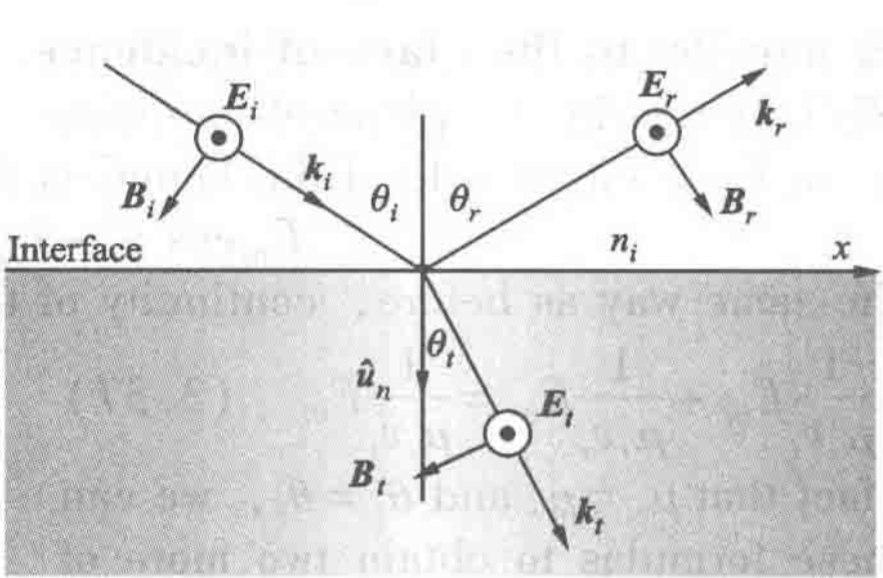
\includegraphics[width=0.5\linewidth]{figures/Fresnel-perpendicular}
  \label{fig:}
\end{figure}

\begin{equation*}
 \left\{
  \begin{aligned}
    & E_i + E_r = E_t \\
    & B_i \cos \theta_i = B_r \cos \theta_r + B_t \cos \theta_t
  \end{aligned}
  \right.
\end{equation*}

\begin{equation*}
  \left\{
  \begin{aligned}
    & E = v B \\
    & v = \dfrac{c}{n}
  \end{aligned}
  \right.
\end{equation*}

We define the amplitude reflection coefficient $r$, the amplitude transmission coefficient $t$

\begin{equation*}
  \begin{aligned}
    r = \dfrac{n_i \cos \theta_i - n_t \cos \theta_t}{n_i \cos \theta_i + n_t \cos \theta_t} \\
    t = \dfrac{2 n_i \cos \theta_i}{n_i \cos \theta_i + n_t \cos \theta_t} 
  \end{aligned}
\end{equation*}

Considered that $n_i \sin \theta_i = n_t \sin \theta_t$

\begin{equation*}
  \begin{aligned}
    r_{\perp} &= \dfrac{\sin \left( \theta_i - \theta_t \right)}{\sin \left( \theta_i + \theta_t \right)} \\
    t_{\perp} &= \dfrac{2 \sin \theta_t \cos \theta_i}{\sin \left( \theta_i + \theta_t \right)} 
  \end{aligned}
\end{equation*}

\subsection{Electric Field Parallel to Plane of Incidence}

\begin{figure}[H]
  \centering
  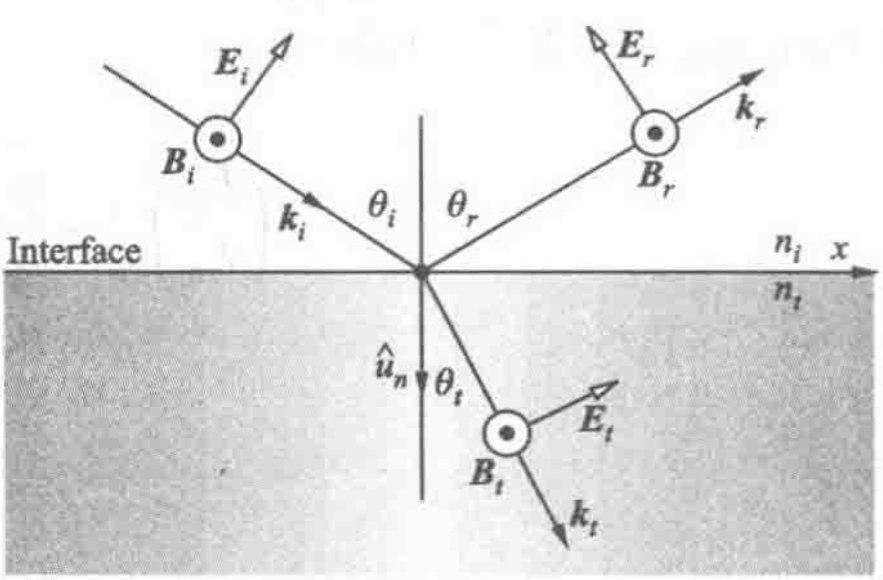
\includegraphics[width=0.5\linewidth]{figures/Fresnel-parallel}
  \label{fig:}
\end{figure}

\begin{equation*}
 \left\{
  \begin{aligned}
    & B_i + B_r = B_t \\
    & E_i \cos \theta_i = E_r \cos \theta_r + E_t \cos \theta_t
  \end{aligned}
  \right.
\end{equation*}

\begin{equation*}
  \left\{
  \begin{aligned}
    & E = v B \\
    & v = \dfrac{c}{n}
  \end{aligned}
  \right.
\end{equation*}

We define the amplitude reflection coefficient $r$, the amplitude transmission coefficient $t$

\begin{equation*}
  \begin{aligned}
    r = \dfrac{n_t \cos \theta_i - n_i \cos \theta_t}{n_t \cos \theta_i + n_i \cos \theta_t} \\
    t = \dfrac{2 n_i \cos \theta_i}{n_t \cos \theta_i + n_i \cos \theta_t} 
  \end{aligned}
\end{equation*}

Considered that $n_i \sin \theta_i = n_t \sin \theta_t$

\begin{equation*}
  \begin{aligned}
    r_{\parallel} &= \dfrac{\sin \left( 2 \theta_i \right) - \sin \left( 2 \theta_t \right)}{\sin \left( 2 \theta_i \right) + \sin \left( 2 \theta_t \right)} = \dfrac{\tan \left( \theta_i - \theta_t \right)}{\tan \left( \theta_i + \theta_t \right)} \\
    t_{\parallel} &= \dfrac{2 \sin \theta_t \theta_i}{\sin \left( \theta_i + \theta_t \right) \cos \left( \theta_i - \theta_t \right)} 
  \end{aligned}
\end{equation*}

\section{Polarization Angle}

\begin{equation*}
  \begin{aligned}
    \theta_p = \arctan \left( \dfrac{\theta_p}{\theta_i}  \right)
  \end{aligned}
\end{equation*}

\begin{figure}[H]
  \centering
  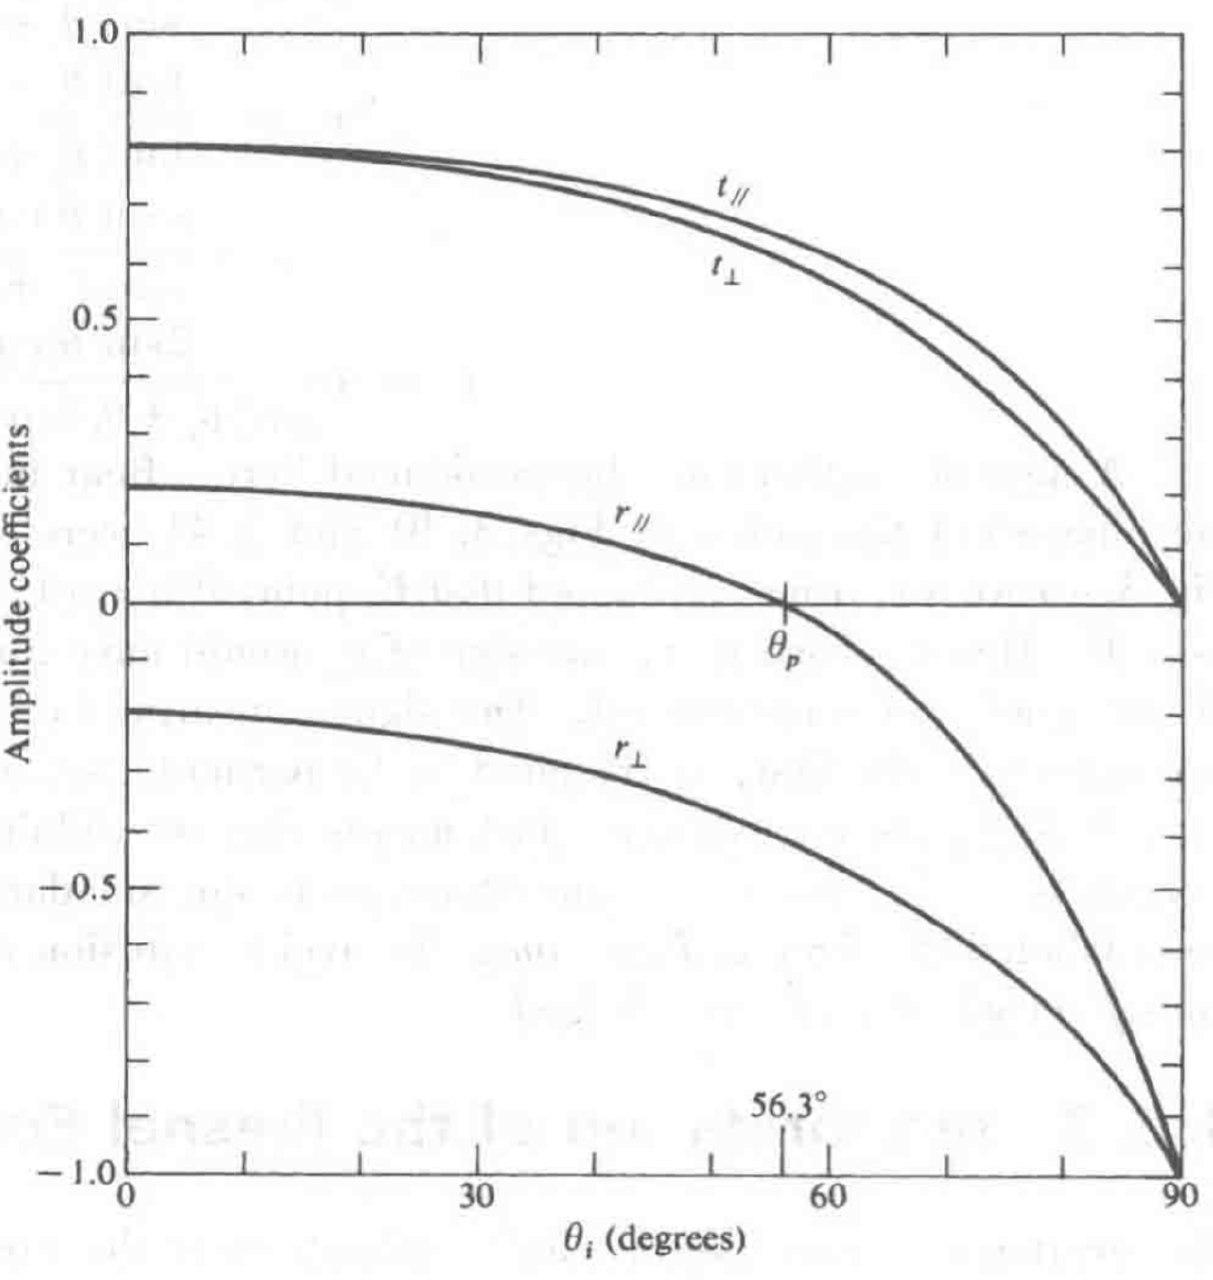
\includegraphics[width=0.3\linewidth]{figures/Polarization-angle}
  \label{fig:}
\end{figure}

\section{Critical Angle}

\begin{equation*}
  \begin{aligned}
    \theta_c = \arcsin \left( \dfrac{n_t}{n_i}  \right)
  \end{aligned}
\end{equation*}

\section{Phase Shift}

When $\theta_i = 0$

\begin{equation*}
  \begin{aligned}
    r_{\perp} &= - r_{\parallel} = \dfrac{n_i - n_t}{n_i + n_t} \\
    t_{\parallel} &= \phantom{+} t_{\perp} = \dfrac{2 n_i}{n_i + n_t} 
  \end{aligned}
\end{equation*}

While $n_i > n_t$ (Inner reflection)

\begin{equation*}
  \begin{aligned}
    r_{\parallel} &< 0 \\
    r_{\perp} &> 0
  \end{aligned}
\end{equation*}

No phase shift.

While $n_i < n_t$ (Outer reflection)

\begin{equation*}
  \begin{aligned}
    r_{\parallel} &> 0 \\
    r_{\perp} &< 0
  \end{aligned}
\end{equation*}

Phase shifted by $\pi$.

\section{Reflectance and Transmittance}

\begin{figure}[H]
  \centering
  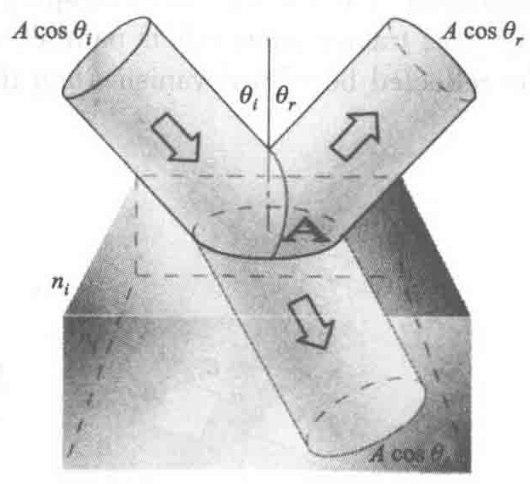
\includegraphics[width=0.4\linewidth]{figures/Reflectance and Transmittance}
  \label{fig:}
\end{figure}


\begin{equation*}
  \left\{
  \begin{aligned}
    R &= \dfrac{I_t A \cos \theta_r}{I_i A \cos \theta_i} = \dfrac{I_t}{I_i} \\
    T &= \dfrac{I_t A \cos \theta_t}{I_i A \cos \theta_i} = \dfrac{I_t \cos \theta_t}{I_i \cos \theta_i}
  \end{aligned}
  \right.
\end{equation*}
\begin{equation*}
  \begin{aligned}
    I = \dfrac{1}{2} \varepsilon v E_0^2 = \dfrac{1}{2} \varepsilon_0 \varepsilon_r v E_0^2 = \dfrac{1}{2} \varepsilon_0 n^2 v E_0^2 = \dfrac{1}{2} \varepsilon_0 n c E_0^2
  \end{aligned}
\end{equation*}

\begin{equation*}
  \left\{
  \begin{aligned}
    R &= \dfrac{I_t}{I_i} = \left( \dfrac{E_{0t}}{E_{0i}}  \right)^2 = r^2 \\
    T &= \dfrac{I_t \cos \theta_t}{I_i \cos \theta_i} = \left( \dfrac{n_t \cos \theta_t}{n_i \cos \theta_i}  \right) \left( \dfrac{E_{0t}}{E_{0i}}  \right)^2 = \left( \dfrac{n_t \cos \theta_t}{n_i \cos \theta_i}  \right) t^2
  \end{aligned}
  \right.
\end{equation*}

\section{The Evanescent Wave}

\begin{figure}[H]
  \centering
  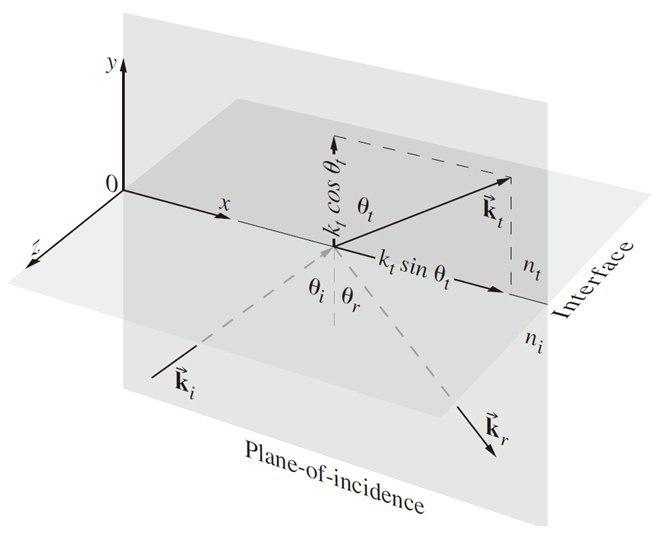
\includegraphics[width=0.5\linewidth]{figures/Evanescent wave}
  \label{fig:}
\end{figure}

\begin{equation*}
  \begin{aligned}
    \vec{E}_t = \vec{E}_{0t} \exp \left[ i \left( \vec{k}_t  \cdot \vec{r} - \omega t \right) \right]
  \end{aligned}
\end{equation*}

\begin{equation*}
  \begin{aligned}
    \vec{k}_t \cdot \vec{r} = k_{tx} x + k_{ty} y
  \end{aligned}
\end{equation*}

\begin{equation*}
  \begin{aligned}
    k_{tx} &= k_t \sin \theta_t = \left( \dfrac{n_i}{n_t}  \right) k_t \sin \theta_i = n_i k_0 \sin \theta_i \\
    k_{ty} &= k_t \cos \theta_t = i k_t \sqrt{\dfrac{n_i^2 \sin^2 \theta_i}{n_t^2} - 1} = i \beta
  \end{aligned}
\end{equation*}

\begin{equation*}
  \begin{aligned}
    \vec{E}_t = \vec{E}_{0t} \exp \left( - \beta y \right) \exp \left[ i \left( n_i k_0 x \sin \theta_i - \omega t \right) \right]
  \end{aligned}
\end{equation*}

\section{Optical Properties of Metals}

The index of refraction of metal is complex

\begin{equation*}
  \begin{aligned}
    \tilde{n} = n_R - i n_I
  \end{aligned}
\end{equation*}

\begin{equation*}
  \begin{aligned}
    \nabla \times \vec{H} = \varepsilon_0 \varepsilon_r \dfrac{\partial \vec{E}}{\partial t} + \sigma \vec{E} = - i \omega \varepsilon_0 \varepsilon_r \vec{E} + \sigma \vec{E} = - i \omega \varepsilon_0 \tilde{\varepsilon}_r \vec{E}
  \end{aligned}
\end{equation*}

Whereas

\begin{equation*}
  \begin{aligned}
    \tilde{\varepsilon}_r = \varepsilon_r + i \dfrac{\sigma}{\omega \varepsilon_0} 
  \end{aligned}
\end{equation*}

\begin{equation*}
  \begin{aligned}
    \tilde{n}^2 = \tilde{\varepsilon}_r = \varepsilon_r + i \dfrac{\sigma}{\omega \varepsilon_0} = \left( n_R + i n_I \right)^2
  \end{aligned}
\end{equation*}

Since $\dfrac{\sigma}{\omega \varepsilon_0 \varepsilon_r} \gg 1 $

\begin{equation*}
  \begin{aligned}
    n_I \approx n_R = \sqrt{\dfrac{\sigma}{2 \omega \varepsilon_0} }
  \end{aligned}
\end{equation*}

Skin depth

\begin{equation*}
  \begin{aligned}
    \delta = \sqrt{\dfrac{1}{2 \omega \mu_0 \sigma} }
  \end{aligned}
\end{equation*}

Reflectance

\begin{equation*}
  \begin{aligned}
    R = \left| \dfrac{n_i - n_t}{n_i + n_t}  \right|^2 = \left( \dfrac{\tilde{n} - 1}{\tilde{n} + 1}  \right) \left( \dfrac{\tilde{n} - 1}{\tilde{n} + 1}  \right)^{*} = \dfrac{\left( n_R - 1 \right)^2 + n_I^2}{\left( n_R + 1 \right)^2 + n_I^2} 
  \end{aligned}
\end{equation*}




%%% Local Variables:
%%% mode: latex
%%% TeX-master: "Optics"
%%% End:
